\chapter{MAC Protocol}
\section{The Problem}
There are t
A naive approach to message passing in a network will 


% Protocols based on transmission schedules    collision-free 
%  resource-inefficient 
%  may require well synchronized nodes throughout the network    difficult to adapt to changing topologies 
%Fundamentals of Wireless Sensor Networks: Theory and Practice Waltenegus Dargie and Christian Poellabauer © 2010 John Wiley & Sons Ltd.
%127 
%        Summary
%  Protocols that let nodes compete for access to the medium 
%  more flexible (easily accommodate changing network topologies)    require less overhead 
%  not collision-free 
%  must possess features that allow them to recover from collisions     network utilization may suffer when collisions occur frequently 


Provided that all nodes are within range of one another, with the use of \ac{cad} before transmissions, and ensuring that transmissions do not occur when a transmitter already has synchronisation \cite{3YP:LORA_SX12}, the vulnerable transmission collision period is very short. In fact collisions should only occur if \ac{cad}s of two transmitters overlap. Unfortunately, it is clear from \ac{phy} testing that for sparse scenarios, whether the environment has high propagation or not, \ac{lora} cannot deliver the required performance to achieve full coverage. This leads to the requirement of handling multi-hop communications and mitigating collisions due to the hidden node problem (highlighted in Figure \ref{fig:hidden_node_problem}).

Mobile-LMAC is a time division approach that can adapt transmission slots dynamically, however there is no mechanism to adjust 

 that would allow all robots to be within a single hop of one another. 


This leads to the requirement of multi-hop communications and handling of the significant challenges they present, namely: collisions (Section \ref{sec:lora_considerations}) in the presence of the hidden node problem (highlighted in Figure \ref{fig:collisions}) and routing (Section \ref{sec:adhocnetworks}). 


Uses Demand Assigned Multiple Access, relies on the fact that there are many channels and low probability of getting the same band, low spreading factors keep localisation where possible, and avoid conflicts with high spreading factor long range transmissions.

First check band that you're going to send in
Use knowledge of who is around from regular broadcasts on 1 band
Send out broadcast with slots for people to reply with CTR on other band (clear to receive)
Send out ATT (about to transmit)
Switch to lower sf and other band




%The \ac{csma} methods introduced in Section are unable to avoid all collisions in a multi-hop network due to the hidden node problem highlighted in Figure .



Can use any RTS, CTS layer
LoRa packets are limited to 255 bytes, but as shown by PHY testing, the shorter the packet, the more reliable it is.
Unable to exploit use of spreading factors as agreement must be made to change settings globally

%Unfortunately, CA does not effectively avoid all collisions in a multi-hop network. In the first place it is not usable when broadcasting, and so it cannot be used, for example, to improve traditional flooding broadcasting. In addition, the interference range of a node is usually greater than its trans- mission range. Specifically, a radio receiver can only decode a signal if the signal power exceeds a minimum threshold, and if the signal power is at least a given factor greater than the noise or interference power. Assume an intended receiver sends a CTS to ask all its neighbors to remain quiet during the upcoming transmission. A node that is just out of range of this receiver does not decode it, and is unaware that a transmission is in progress, and so proceeds to transmit its own packet. Although the node is too distant to directly communicate with the receiver, the strength of its trans- mission (which is noise to the receiver, which is listening to a different packet) may reduce the signal-to-noise ratio at the receiver enough that the receiver is unable to decode its incoming packet. Although it is a matter of semantics whether this should be classified as interference or collision, it is clear that even for unicast transmission CA does not always prevent one node’s communication from interfering with communication among other nodes.




When always within range the 
but also identifies a significant collision challenge caused by standard ALOHA protocols. THe 

Better to keep low duty cycle, 10\% will have massive collisions
From PHY testing it is known that 
Also know that if devics are moving, LOS changes in forests may suddenly cause packet failure, better to shove all data asap
 
Use 11, 9, 8, 7
Collision avoidance using channel sensing (e.g. via \ac{cad})

This will be extremely prevalent if there is a high 

By not focusing on power reduction, the high number of packets of adr is not requied.

single hop behaviour would no


Based on the physical performance in the environment about radio behaviour and imposed constraints from the theroetical about the technology  

Mainly target the local broadcast idea introduced in the introduction
Also consider how it can be adapted to  the other scenarios


It is unreasonable to expect 
% Coping with hops, on demand (reactive) or table driven (proactive), (minimise need but use AODV or DSR). 
%LoRa packets can only be 256 bytes (due to FIFO buffer size, see official documentation https://www.semtech.com/products/wireless-rf/lora-transceivers/SX1276).
%LoRa packet transmit time ranges from 200ms to 1s depending on packet size.\
%https://github.com/sudomesh/disaster-radio/wiki/Protocol
\section{Proposal}

Phy testing has shown that distance cannot be covered by a gateway
Proposed solution is agnostic to routing protocol

% Duty cycles (decided on method [manage per hour])
% Bands (dual band)
% Message types
% PHY layer parameter selection
% Adaptiveness???
% a461331.pdf general collision avoidance
%


 


% have robot knowing whos around from frequent packet updates
% robot can then decide on sending parameters before sending request

\section{Duty Cycle}
\begin{figure}[H]
    \centering
   	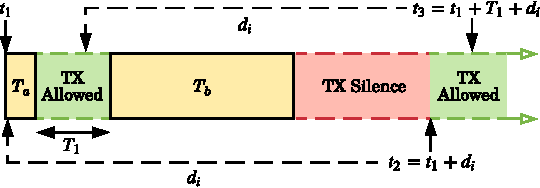
\includegraphics{Figures/duty_cycle_proposed.pdf}
    \caption[Proposed duty cycle enforcement method]{
    Demonstration of proposed method for duty cycle limit enforcement. Unlike \ac{lorawan}'s method the behaviour can vary greatly depending on when transmissions occur and how long they are, therefore this diagram is only a partial representation. It is valid provided there are no transmissions since $t=t_1-d_i$, where $d_i$ is the duty cycle interval (e.g. 3600 seconds). The duty cycle ($d_c$) shown is $\frac{T_a + T_b}{d_i}$. Enforcement is handled as follows. Immediately after the first transmission occurs, the remaining interval allowance is $T_b$ ($T_a+T_b-T_a$). This could be used immediately but, for purposes of demonstration, a short period of silence occurs. Once the transmission of length $T_b$ occurs, the remaining interval allowance is 0 ($T_b - T_b$), therefore the transmitter must be silent until allowance is freed. At $t_2$ a transmission of length $T_a$ would be allowed because for every time unit of a new transmission, the corresponding time unit of $T_a$ would no longer fall in the time interval. A longer transmission would not be allowed until $t_3$ because $T_b$ will not fall outside of the time interval until $T_1$ has elapsed. Note that as $T_a$ is already available the transmission can start $T_a$ before $T_b$ actually falls out of the interval. Therefore at $t_3$ a transmission of $T_a + T_b$ would be allowed (in this case, the full interval limit). The figure is not to scale.    
    }
    \label{fig:proposed_duty_cycle}
\end{figure}



Duty cycle:
Can quickly get complicated to understand when dealing with more complex transmission scenarios  (e.g. short send, wait, short send, wait, long send, etc...). However, simple to implement using a linked list, which gets culled when a send needs to occur. Delete old entries and find overlaps with current time - di. Can start sending as soon as the previous transmission started. Though processing intensive, allows predictable scheduling.

